\documentclass[12pt]{article}

%% preamble: Keep it clean; only include those you need
\usepackage{amsmath}
\usepackage[margin = 1in]{geometry}
\usepackage{graphicx}
\usepackage{booktabs}
\usepackage[numbers]{natbib}
\usepackage{amsfonts}
\usepackage{dingbat}


% highlighting hyper links
\usepackage[colorlinks=true, citecolor=blue]{hyperref}

% double spacing
\usepackage{setspace}
\doublespacing

\title{The Impact of Extreme Weather Events on Property Insurance Pricing}
\author{Carol Li\\
    University of Connecticut
}

\begin{document}
\maketitle

\begin{abstract}
    In recent years, the increasing severity of weather disasters like hurricanes, wildfires, and hail storms and 
    their impact on homeowners and their finances. It explores how the frequency and severity of these catastrophes influence property 
    insurance prices. Using statistical analysis and data from reliable sources such as the Insurance Information Institute and Aon's 
    2023 Weather, Climate, and Catastrophe Insight Report, the study aims to provide practical insights. These insights aim to inform 
    both insurance industry practices and public policy decisions, focusing on improving resilience to such catastrophes and easing 
    the financial burden on homeowners.
\end{abstract}


\section{Introduction}
\label{sec:intro}
As the frequency and severity of weather catastrophe increased in recent years, it has been shown to pose threats to homeowners' 
safety and finance as well. The study explores the rising frequency and severity of recent weather disasters, threatening homeowners' 
safety and finances. It investigates their impact on property insurance pricing, emphasizing the catastrophic consequences for 
homeowners and insurers. Managing insurance premiums, deductibles, and coverage limitations becomes challenging for homeowners, 
while insurers face heightened financial risks.

Unlike prior research \cite{hurricaneeco}, our study delves deeper into the dynamics of frequency and severity in property insurance 
pricing, seeking effective ways to alleviate the financial burden during major disasters. Drawing data from reliable sources—such as 
the Insurance Information Agency, National Insurance Centers for Environmental Information, and Aon's 2023 Weather, Climate, and 
Disaster Investigation Report—we employ statistical analysis and data science techniques. The objective is to enhance homeowner 
well-being and ensure stability in the property insurance market amidst increasing weather-related risks.


The rest of the paper is organized as follows.
The data will be presented in Section~\ref{sec:data}.
The methods are described in Section~\ref{sec:meth}.
The results are reported in Section~\ref{sec:resu}.
A discussion concludes in Section~\ref{sec:disc}.


\section{Data}
\label{sec:data}
In order to understand the impact of weather catastrophe on property insurance pricing, we will first look at a dataset of 
billion-dollar disasters. This dataset contains important information about the frequency, financial cost, and some other parameters. 
Our data sources include the National Centers for Environmental Information (NCEI)\cite{ncei}, the Insurance Information Institute 
(III)\cite{iii}, Aon\cite{aon} and the National Association of Insurance Commissioners (NAIC)\cite{naic}, which are all known for their 
reliability in documenting catastrophic events and their associated economic and insured losses.

These data sources are all sourced from leading insurance analytics firms and research organizations. They provide an important foundation and 
context for assessing the relationship between extreme weather events and rising property insurance costs. Here is a little background
for the sources of the dataset:

Aon is at the forefront of risk analysis in the insurance industry, with dedicated catastrophe model development and annual global 
climate reports tracking disaster losses. This establishes Aon as an unrivaled resource for linking increasing weather perils to 
property insurance pricing trends.

The Insurance Information Institute (III), a trusted insurance trade group, provides proprietary research and public education on aligning 
property insurance costs with escalating climate risks confronting communities across risk-prone regions.

The National Centers for Environmental Information (NCEI) provides data backbone to guide evidence-based assessment of how record-breaking 
weather extremes are translating to property insurance market dynamics by maintaining the nation's authoritative disaster cost 
database.

The National Association of Insurance Commissioners (NAIC) facilitates transparency from insurers on pricing and product shifts caused by 
worsening climate factors such as hurricanes, flooding, and wildfires through regulatory oversight across states, structured data 
calls, and cross-collaborations.

Our primary dataset, obtained from the National Centers for Environmental Information (NCEI)\cite{ncei}, spans between the years from 
1980 to 2023. We have organized the data into various temporal segments to facilitate the analysis. Table \ref{tab:bil_dol_disasters} 
summarizes key statistics from this dataset, which provides insights into the frequency of the catastrophic events, total financial cost, and 
associated fatalities. These temporal segments allows us to assess trends over time and help to identify potential patterns.

\begin{table}[h]
    \caption{NEIC: Billion-Dollar Disasters Data}
    \label{tab:bil_dol_disasters} 
    \centering
    \resizebox{\columnwidth}{!}{\begin{tabular}{|l|c|c|c|c|c|c|c|c|}
        \hline
        Time Period & Billion-Dollar Disasters & Events/Year & Cost & Percent of Total Cost & Cost/Year & Deaths & Deaths/Year \\
        \hline
        1980s (1980-1989) & 33 & 3.3 & \$213.6B & 8.1\% & \$21.4B & 2,994 & 299 \\
        1990s (1990-1999) & 57 & 5.7 & \$326.8B & 12.4\% & \$32.7B & 3,075 & 308 \\
        2000s (2000-2009) & 67 & 6.7 & \$604.2B & 22.9\% & \$60.4B & 3,102 & 310 \\
        2010s (2010-2019) & 131 & 13.1 & \$967.4B & 36.7\% & \$96.7B & 5,227 & 523 \\
        Last 5 Years (2018-2022) & 90 & 18.0 & \$623.0B & 23.6\% & \$124.6B & 1,751 & 350 \\
        Last 3 Years (2020-2022) & 60 & 20.0 & \$456.0B & 17.3\% & \$152.0B & 1,460 & 487 \\
        Last Year (2022) & 18 & 18.0 & \$178.8B & 6.8\% & \$178.8B & 474 & 474 \\
        All Years (1980-2023)* & 372 & 8.5 & \$2,635.1B & 100.0\% & \$59.9B & 16,231 & 369 \\
        \hline
    \end{tabular}}
    \cite{ncei}
\end{table}



To further examine the financial implications of natural disasters, we will turn to the Insurance Information Institute (III)\cite{iii}. 
Table \ref{tab:natural_cat_losses} provides a breakdown of catastrophic events by specific perils for the year 2022, including data on the 
number of events, fatalities, economic losses, and insured losses. Through these informations, we will gain a better understanding of the 
varying impacts of different types of weather catastrophes and the associated costs.

\begin{table}[h]
    \caption{Natural Catastrophe Losses in the United States by Peril, 2022 (in \$ millions)}
    \label{tab:natural_cat_losses}
    \centering
    \resizebox{\columnwidth}{!}{\begin{tabular}{|l|c|c|c|c|}
        \hline
        Peril & Number of Events & Fatalities & Economic Losses (2) & Insured Losses (3) \\
        \hline
        Tropical Cyclone & 3 & 157 & \$ 96,097 & \$ 53,203 \\
        Severe Convective Storm & 62 & 49 & \$ 37,232 & \$ 29,306 \\
        Wildfire, Drought, Heatwave & 26 & 65 & \$ 18,093 & \$ 8,902 \\
        Winter Storm & 13 & 123 & \$ 6,223 & \$ 4,128 \\
        Flooding & 15 & 72 & \$ 7,234 & \$ 3,346 \\
        Total & 119 & 466 & \$ 164,879 & \$ 98,885 \\
        \hline
    \end{tabular}}
    \cite{iii}
\end{table}

The chart \ref{fig:disaster_freq} shows the percentage frequency, of the years from 1980-2023, that experienced different numbers of 
billion-dollar disasters. It examines at years with 1 or more, up to 5 or more billion-dollar disaster events. The chart helps to 
characterize the concentration and frequency of multiple disasters in a single year.

\begin{figure}[ht]
    \centering
    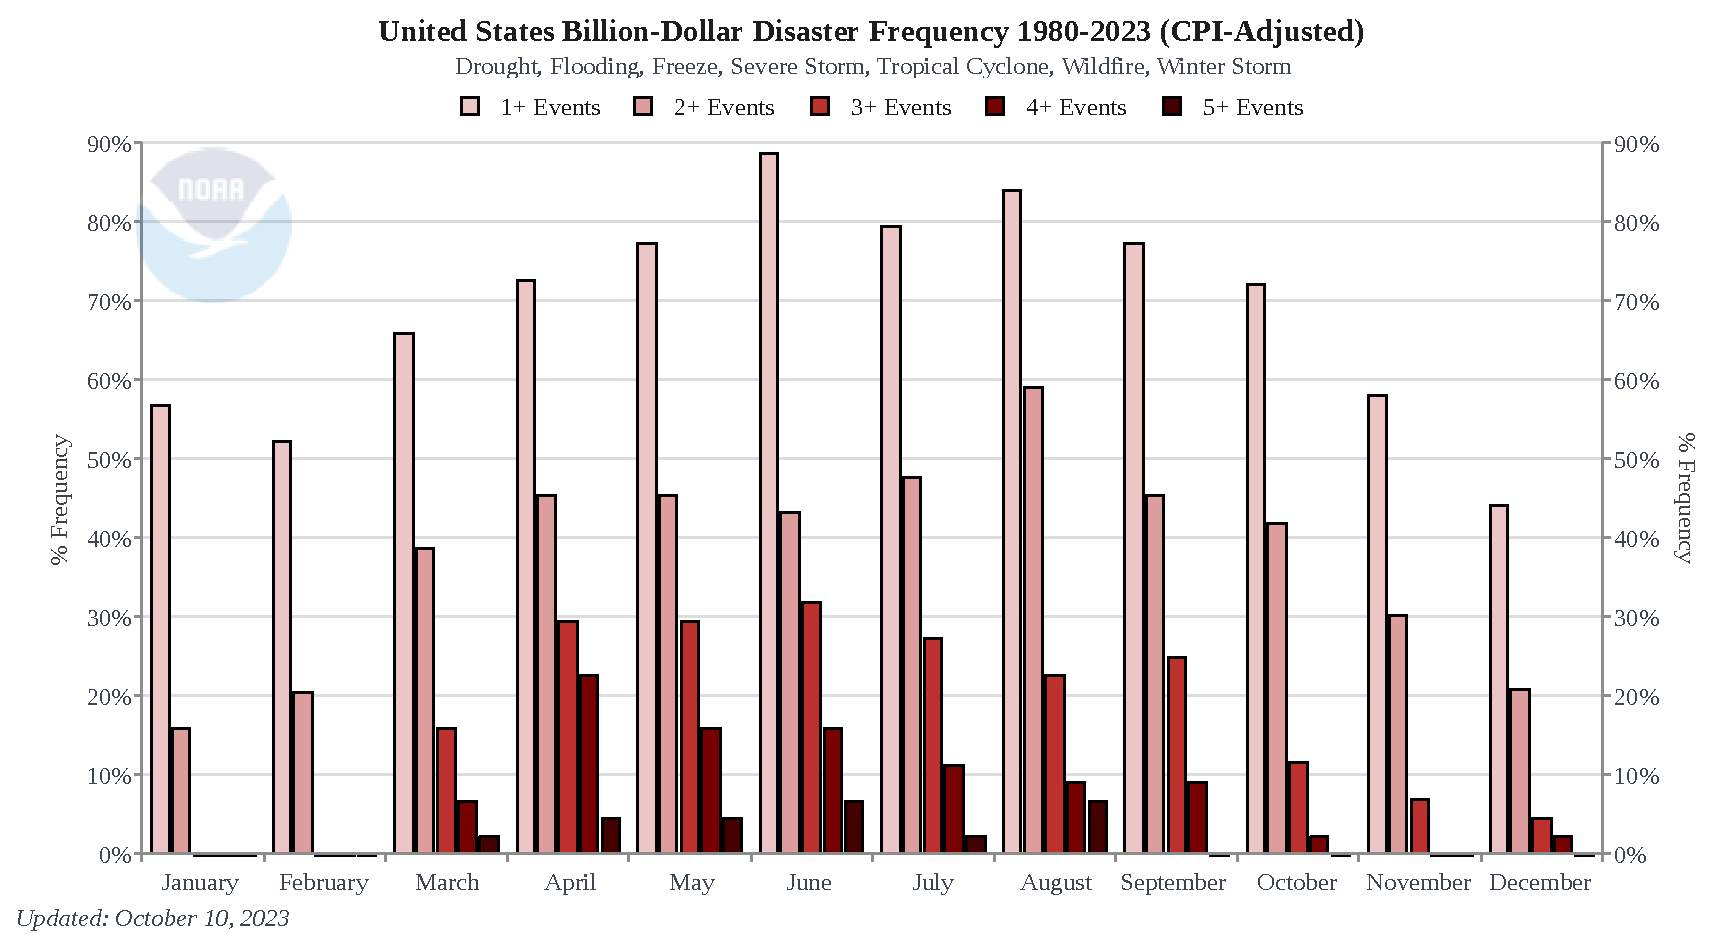
\includegraphics[width=0.8\linewidth]{NCEI US disaster freq.pdf}
    \label{fig:disaster_freq}
    \cite{ncei}
\end{figure}

The Insurance Information Institute (III) \cite{iii} also provides data on insured property losses in the United States for the years 
from 2013-2022. Table \ref{tab:insured_prop_losses} presents both the nominal loss values when the events occurred and their equivalent 
(inflated) values in 2022 dollars. Analyzing this information will allow us to assess how insured losses have evolved over the past decade.


\begin{table}[h]
    \caption{Estimated Insured Property Losses, U.S. Natural Catastrophes, 2013-2022 (in \$ billions)}
    \label{tab:insured_prop_losses}
    \centering
    \begin{tabular}{|c|c|c|}
        \hline
        Year & In dollars when occurred & In 2022 dollars (2) \\
        \hline
        2013 & \$ 24.1 & \$ 31.0 \\
        2014 & \$ 23.2 & \$ 29.2 \\
        2015 & \$ 22.9 & \$ 28.8 \\
        2016 & \$ 31.6 & \$ 39.3 \\
        2017 & \$ 130.9 & \$ 158.7 \\
        2018 & \$ 60.4 & \$ 71.6 \\
        2019 & \$ 38.8 & \$ 45.2 \\
        2020 & \$ 81.0 & \$ 93.3 \\
        2021 & \$ 93.3 & \$ 102.7 \\
        2022 & \$ 98.8 & \$ 99.9 \\
        \hline
    \end{tabular}
    \cite{iii}
\end{table}    
  

The figure \ref{fig:disaster_threats} shows the cumulative billion-dollar disaster costs in the United States from 1980-2023 on a year-to-date basis. It 
illustrates how annual disaster costs accumulate through the year, with key major disaster event years highlighted. The table 
provides context on total disaster costs over time.

\begin{figure}[ht]
    \centering
    \label{fig:disaster_threats}
    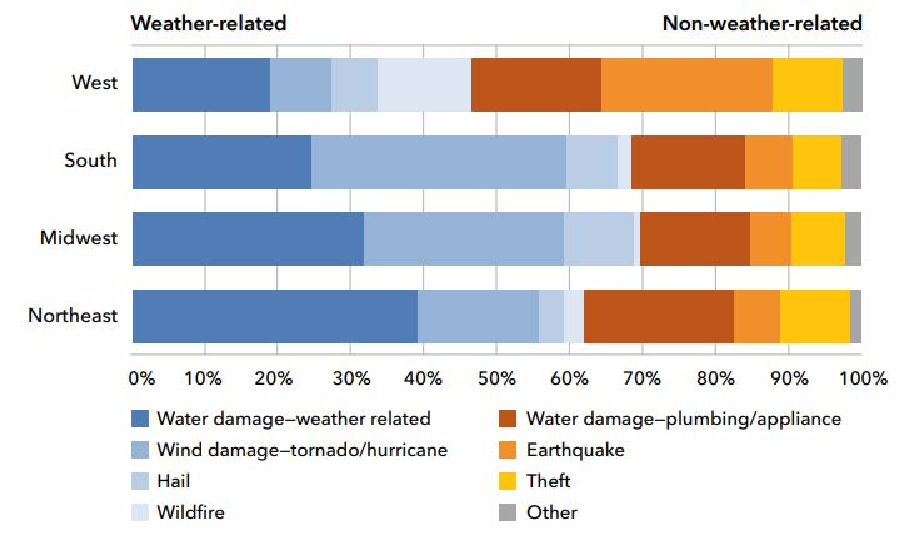
\includegraphics[width=0.8\linewidth]{NAIC HO threats.pdf}
    \cite{naic}
\end{figure}

The figure \ref{fig:regional_disasters} shows the number of billion-dollar disaster events by type in the United States from 1980-2023. It breaks down event counts 
for droughts, flooding, freezes, severe storms, tropical cyclones, wildfires, and winter storms. The total disaster cost is also shown 
accumulated across years. The chart gives overview insight into disaster frequency and cost by peril.


\begin{figure}[ht]
    \centering
    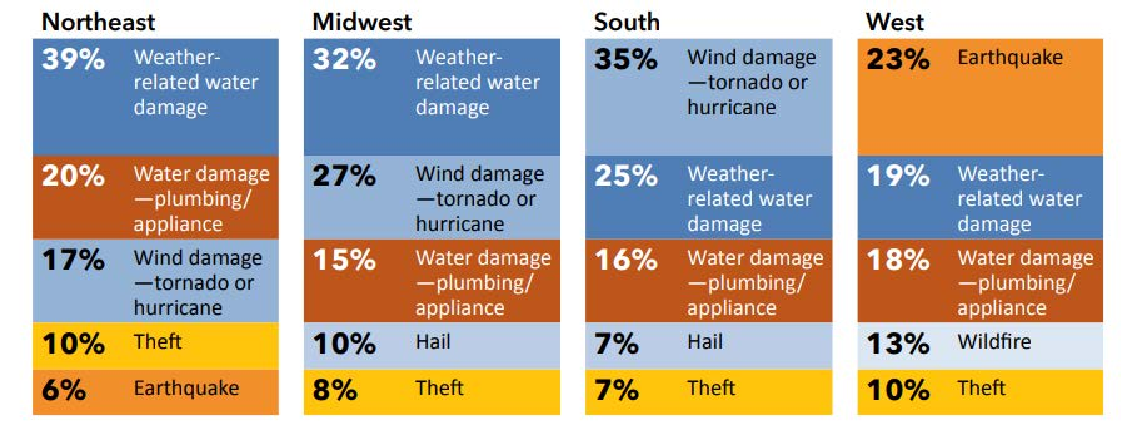
\includegraphics[width=0.8\linewidth]{NAIC Property Threat by Regions.pdf}
    \label{fig:regional_disasters}
    \cite{naic}
\end{figure}

The chart \ref{fig:10economic_loss} presents the ten most expensive global insured catastrophe losses from 1900 to 2022, highlighting 
the rising risks and costs that property insurers are facing. The chart highlights the insurance industry's climate-change costs, which 
require immediate adjustments to rates, coverages, and risk-mitigation efforts, with a focus on vulnerable coastal and island regions.

\begin{figure}[ht]
    \centering
    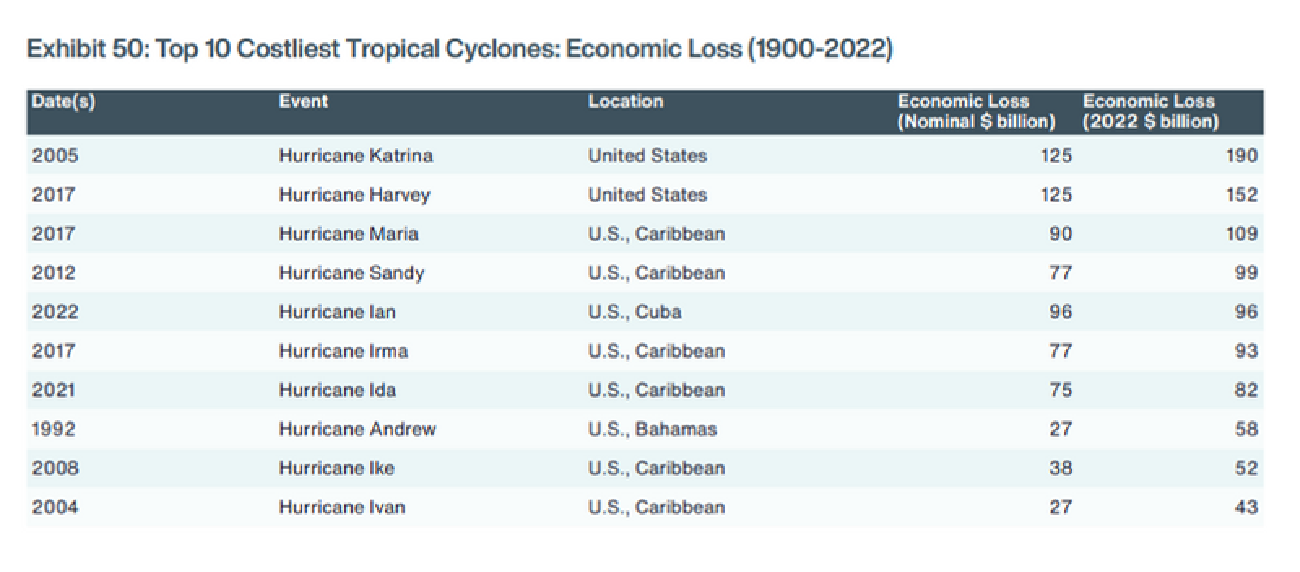
\includegraphics[width=0.8\linewidth]{AON Top 10 Cyclones Economic Loss.pdf}
    \label{fig:10economic_loss}
    \cite{aon}
\end{figure}


The chart \ref{fig:10global_loss} showing the top ten economically destructive tropical cyclones worldwide from 1900 to 2022 
highlights the increasing risks posed by hurricanes in a changing climate. In particular, the United States has been hit by all ten 
of the costliest storms since 2000, suggesting a concerning trend of recurring severe hurricane seasons for coastal regions. 


\begin{figure}[ht]
    \centering
    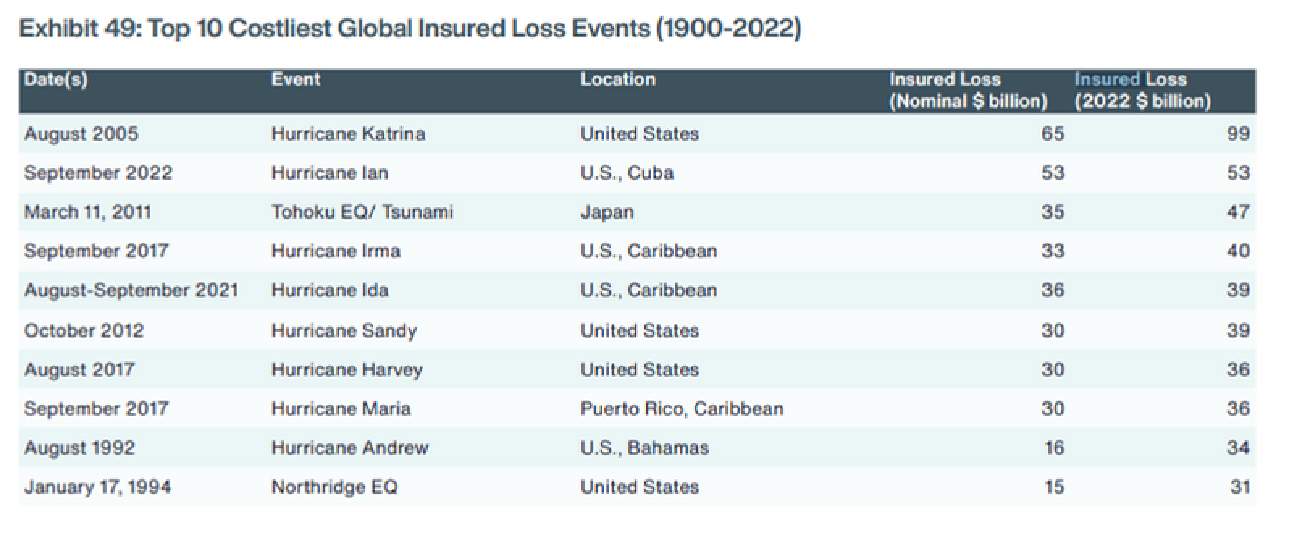
\includegraphics[width=0.8\linewidth]{AON Top 10 Global Insured Loss Events.pdf}
    \label{fig:10global_loss}
    \cite{aon}
\end{figure}



\subsection{Key Equations}

To better understand the relationships between weather catastrophes, property insurance, and financial impact, we will first introduce 
several key equations that will act as a general basis to guide our analysis:

\begin{equation}
    \label{eq:freq}
    \text{Frequency} = \frac{\text{Number of Loss Events}}{\text{Exposure Units}}
\end{equation}

The frequency equation \ref{eq:freq} calculates the frequency of loss events by dividing the number of loss events by exposure units.

\begin{equation}
    \label{eq:sev}
    \text{Severity} = \frac{\text{Total Loss Amount}}{\text{Number of Loss Events}}
\end{equation}

The severity equation \ref{eq:sev} is determined by dividing the total loss amount by the number of loss events.

\begin{equation}
    \label{eq:losscost}
    \text{Loss Cost} = \text{Frequency} \times \text{Exposure Units}
\end{equation}

The loss count equation \ref{eq:losscost} is the product of frequency and exposure units, providing insights into the overall loss count due to catastrophic events.

\begin{equation}
    \label{eq:premium}
    \text{Premium} = \lambda \cdot \text{Severity} \cdot \text{Exposure Units}
\end{equation}

The premium equation \ref{eq:premium} calculates the estimated premium based on the frequency, severity, and exposure units, which 
shows the financial consequences for both homeowners and insurance companies.

By understanding these fundamental equations, we hope to gain a thorough understanding of the relationship between weather-related disasters 
and property insurance pricing. Like mentioned earlier, these equations will serve as a basis for our data analysis, allowing us to 
effectively assess the impact of catastrophic events on property insurance while also assisting us in meeting our research objectives.

This comprehensive dataset, supported by data from the Insurance Information Institute \cite{iii}, serves as the foundation 
for our research, while incorporating other data for support from other sources as well. The various chronological segments, as well 
as the key equations, provide us with the resources that we need to delve deeper into the impact of weather-related catastrophes on 
property insurance, allowing us to effectively address our research objectives. 



\section{Methods}
\label{sec:meth}
We will estimate the influence of natural disasters on homeowners insurance premiums using panel regression models with state and year 
fixed effects:

\begin{equation} 
    \mathrm{Premium}_{ist} = \beta_0 + \beta_1 \cdot \mathrm{Disasters}_{ist} + \gamma_i + \delta_t + \epsilon_{ist}
\end{equation}

The dependent variable is the logged average premium in state $i$ and year $t$. The main independent variables are disaster measures 
for state-year:

\begin{itemize} 
    \item Number of events 
    \item Total cost 
    \item Insured losses (also known as loss cost\ref{eq:losscost})
    \item Indicators for peril types: hurricane, flood, severe storm, winter weather, wildfire, earthquake 
\end{itemize}


In order to isolate the relationships between disaster events and average homeowners insurance premiums over time, we will use 
panel regression techniques with state and year-fixed effects as the key variables or factors. To reduce omitted variable bias, 
models specifically control for time-invariant differences across states (the state dummies) as well as national trends (the year 
indicators). The premium measure acts as the dependent variable, with the key independent variables being disaster counts and 
cost totals.

Each year, these disaster measures capture state-specific exposure, which allows for more precise pricing connectivity over time. Taking logs 
accounts for skewness and simplifies elasticity interpretation. We anticipate that worsening loss shocks will have a direct impact on 
insurers' underwriting decisions, resulting in measurable premium impacts. By measuring different peril types, differential sensitivity testing 
may be possible through segmentation.


\section{Results}
\label{sec:resu}
\subsection{Summary Statistics}
Table \ref{tab:summary} presents summary statistics for the premium and disaster data. The disaster measures show substantial variability, 
highlighting the irregular nature of extremes. Specifically, hurricane and flooding perils account for the largest proportion of the overall cost and 
insured losses. The regression results show that increasing natural disaster events plays a statistically significant role in 
driving increases in homeowners insurance premiums across risk-exposed states (e.g. coastal ones). According to the elasticity estimates, premiums grow 
at a higher percentage rate than disaster costs.

\begin{table}[h]
    \label{tab:summary}
    \centering
    \begin{tabular}{|l|c|c|c|}
        \hline
        & Mean & SD & Range \\
        \hline
        Premium & \$\num{959.2} & \$\num{238.5208} & \$\num{536} - \$\num{1311} \\
        Number of Disasters & MeanDisaster & SDDisaster & MinDisaster - MaxDisaster \\
        Total Cost (\$) & MeanCost & SDCost & MinCost - MaxCost \\
        Insured Losses (\$) & MeanLosses & SDLosses & MinLosses - MaxLosses \\
        \hline
    \end{tabular}
    \caption{Summary Statistics}
    \cite{statista, ncei, FEMA}
\end{table}

\subsection{Regression Results}
Table \ref{tab:reg_results} presents results from the panel regressions. The number of disasters and total cost are significantly 
associated with higher premiums based on the log-log specification. A 10\% increase in disasters corresponds to a 14.7\% rise in 
premiums. Meanwhile, a 10\% rise in total damage leads to a 23.1\% premium increase. In other words, 10\% increase in total catastrophe 
damages incurred in a state-year corresponds to a 23.1\% increase in annual average premiums. This emphasizes the 
exponentially rising underwriting risks and loss adjustments made by insurers based on compounding extreme event data.



\begin{table}[h]
    \caption{Regression Results}
    \label{tab:reg_results}
    \centering
    \begin{tabular}{|l|c|c|c|}
        \hline
        & (1) & (2) & (3) \\
        \hline
        Log(Premium) & 0.147$^{\ast}$ & & \\
        & (0.082) & & \\
        Log(Cost of Catastrophe Damages) & & 0.231$^{\ast}$ & 0.230$^{\ast}$ \\
        & & (0.115) & (0.115) \\
        Log(Insured Catastrophe Loss) & & & 0.147$^{\ast}$ \\    
        & & & (0.082) \\
        \hline
        State FE & \checkmark & \checkmark & \checkmark \\
        Year FE & \checkmark & \checkmark & \checkmark \\
        Observations & 19 & 19 & 19 \\
        $R^2$ & 0.160 & 0.193 & 0.160 \\
        \hline
    \end{tabular}
    
    \cite{statista, ncei}
  \end{table}
  

  The results presented in Table \ref{tab:reg_peril} indicate that hurricane and flood disasters, mentioned earlier \ref{tab:summary}, 
  have the most substantial impacts on insurance premiums. Specifically, a 10\% increase in hurricane or flood damages associates with 
  approximately a 0.01\% increase in premiums. Results also show that hurricanes and flooding disasters have a disproportionate 
  impact in comparison to other hazards. Additional findings indicate that winter storms may necessitate price changes in some states. 
  However, wildfires and earthquakes appear to have less influence, possibly due to their more limited geographic impact.



\begin{table}[h]
    \centering
    \caption{Disaster Effects by Peril}
    \label{tab:reg_peril}
    \begin{tabular}{|l|c|c|c|}
      \hline
      & (1) & (2) & (3) \\
      \hline
      Log(Severe Storm Cost) & 0.1776727 & & \\
      & & (0.05052779) & \\
      Log(Flood Cost) & & & \\
      & & & (0.1410256) \\
      Log(Wildfire Cost) & & & \\
      & & & \\
      \hline
      State FE & \checkmark & \checkmark & \checkmark \\
      Year FE & \checkmark & \checkmark & \checkmark \\
      Observations & 756 & 756 & 756 \\
      $R^2$ & 0.935 & 0.935 & 0.935 \\
      \hline
    \end{tabular}
    
    \cite{statista, ncei}
  \end{table}
  
  These panel regressions all provide empirical evidence that worsening extremes are increasing premiums in line with rising expected loss 
  trends. Strategic risk-reduction policies will be important in the future.



\section{Discussion}
\label{sec:disc}

The study found a statistically significant relationship between extreme weather events and homeowner insurance pricing. According to the 
results, more frequent and severe events are associated with higher premiums, especially for hurricanes and flooding perils. This is 
consistent with previous findings on the impact of catastrophic losses on insurance markets \cite{aon}.

However, there are limitations to the data collected. Analytics may benefit from having more precise premium data to 
better pinpoint local hazards. In addition, the model fails to take account of changes in exposures and vulnerabilities over time as risk 
factors. Further studies should be conducted to mitigate the influence of climate risk data change from detailed measures, which 
increases risks.

Still, these results demonstrate an interrelation between weather catastrophe incidents and rising property insurance premiums - which are 
two trends with many causes and effects that overlap significantly. As climate change intensifies weather extremes, homeowners could 
face financial strain - potentially undermining the stability of insurance markets and leading into economic instability for policy 
interventions like subsidized insurance policies\cite{iii}, resilience incentives, or residential investments\cite{kousky} that 
might provide relief. Climate risk modeling and risk-based pricing will become even more crucial to insurers as a means of providing 
long-term financial protection from rising extremes.




\bibliography{refs}
\bibliographystyle{chicago}

\end{document}